\documentclass[english]{article}
\usepackage[english]{babel} 
\usepackage[T1]{fontenc}
\usepackage[utf8x]{inputenc}
\usepackage{float}
\usepackage{graphicx}

\makeatletter
\usepackage[a4paper,top=2cm,bottom=2cm,left=2cm,right=2cm]{geometry}
\usepackage{enumitem}
\usepackage{subfig}
\usepackage{amsthm}
\usepackage{amsmath}
\usepackage{epstopdf}
\usepackage{fancyhdr}
\usepackage{booktabs,array}

\hyphenation{english}
\makeatother

\usepackage{babel}


\usepackage{listings}
\usepackage{xcolor} % for setting colors

% set the default code style
\lstset{
    frame=tb, % draw a frame at the top and bottom of the code block
    tabsize=4, % tab space width
    showstringspaces=false, % don't mark spaces in strings
    numbers=left, % display line numbers on the left
    commentstyle=\color{gray}, % comment color
    keywordstyle=\color{blue}, % keyword color
    stringstyle=\color{red} % string color
}


\begin{document}
\begin{titlepage}

	\begin{center}
		\begin{Large} \textbf{UNIVERSITY OF PADOVA} \\
		\end{Large} \vspace{1cm}
		\vspace{3cm}
		\begin{Large} Embedded Real--Time Control \end{Large}
		\par\end{center}

	\begin{center}
		\begin{Large}Laboratory report\\
		\end{Large}
		\par\end{center}

	\begin{center}
		\vspace{2cm}
		\begin{figure}[!htb]
			\centering 
\includegraphics[width=8cm]{figures/unipd-logo.png}\\

		\end{figure}

		\par\end{center}

	\begin{center}
		\vspace{2cm}
		\begin{Large} Names - (Student ID Numbers)  \\
		\end{Large} \vspace{2cm}
		\begin{Large} Academic Year 2021-2022 \end{Large}
		\par\end{center}

\end{titlepage}

\tableofcontents
\newpage

\section{Laboratory 1}

In this lab ....

\subsection{Relevant theoretical notions}

Lorem ipsum dolor sit amet, consectetur adipisci elit, sed eiusmod tempor incidunt ut labore et dolore magna aliqua. Ut enim ad minim veniam, quis nostrum exercitationem ullam corporis suscipit laboriosam, nisi ut aliquid ex ea commodi consequatur.

\begin{figure}[!h]
	\centering
	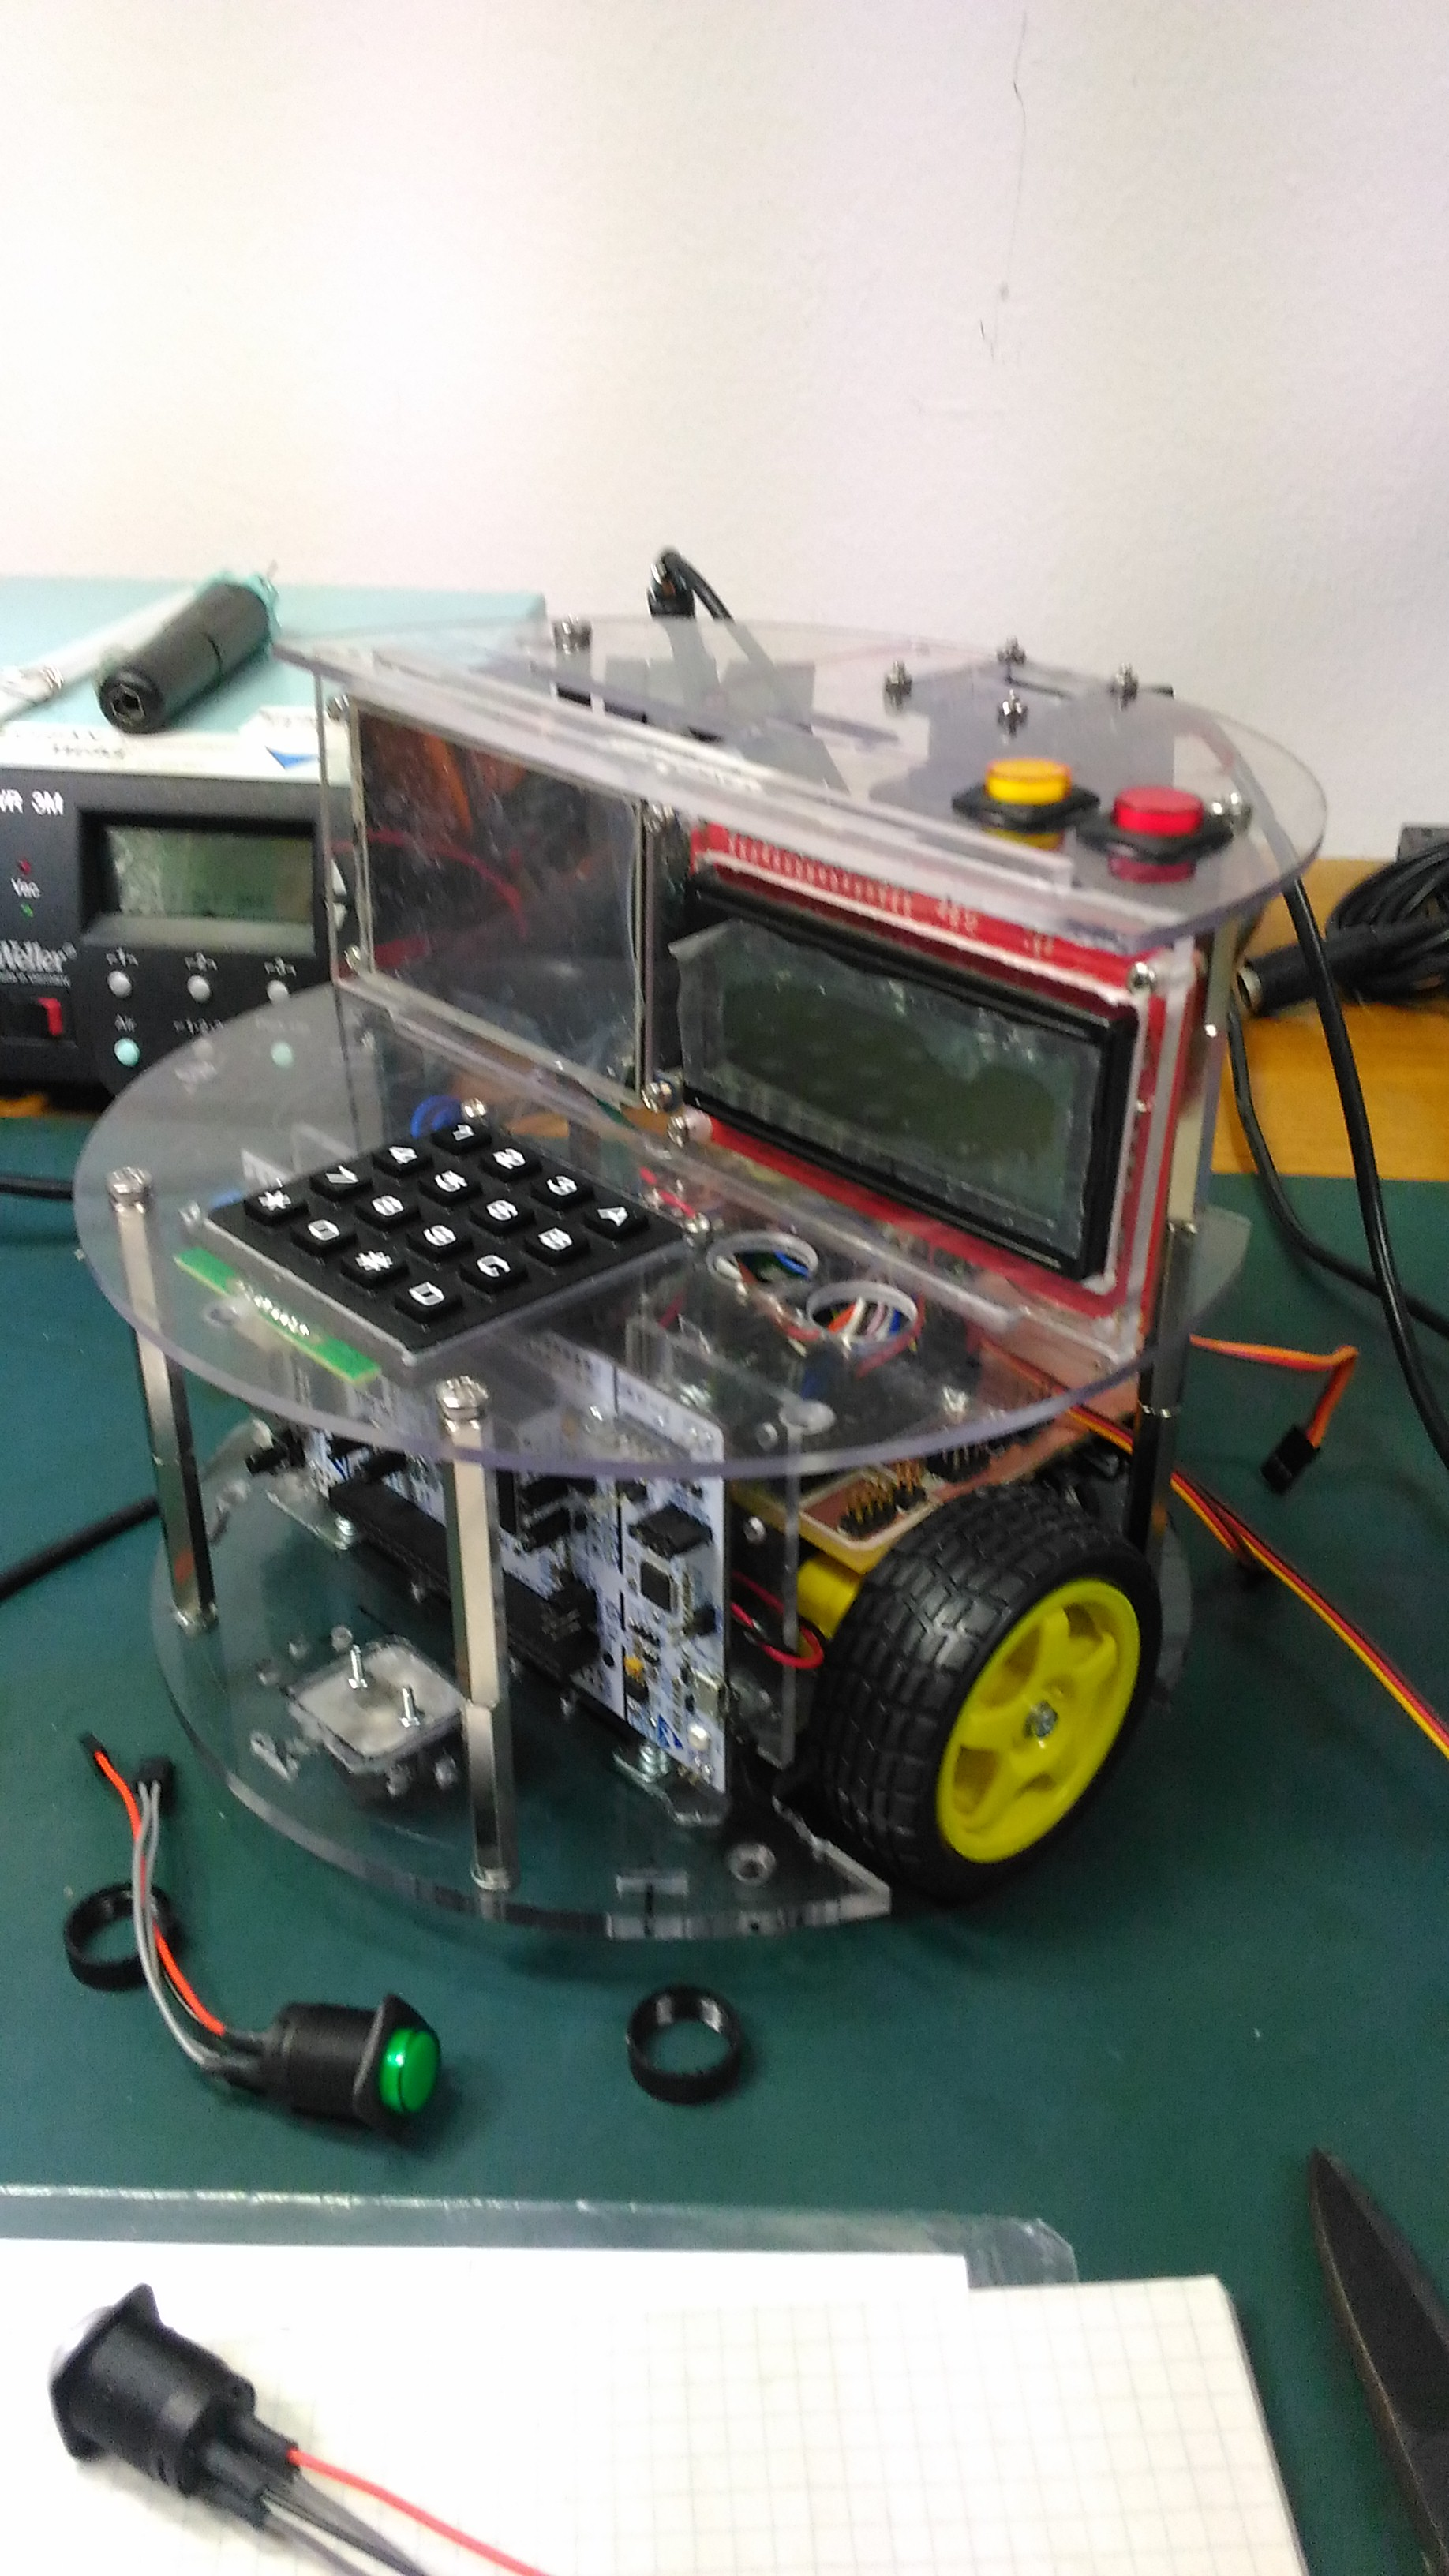
\includegraphics[width=0.4\textwidth]{figures/turtlebot_1.jpg}
	\caption{The TurtleBot}
	\label{fig:turtlebot}
\end{figure}

In Figure~\ref{fig:turtlebot} ...

\begin{figure}[!ht]
	\centering
	\subfloat[The TurtleBot 1 ]
	{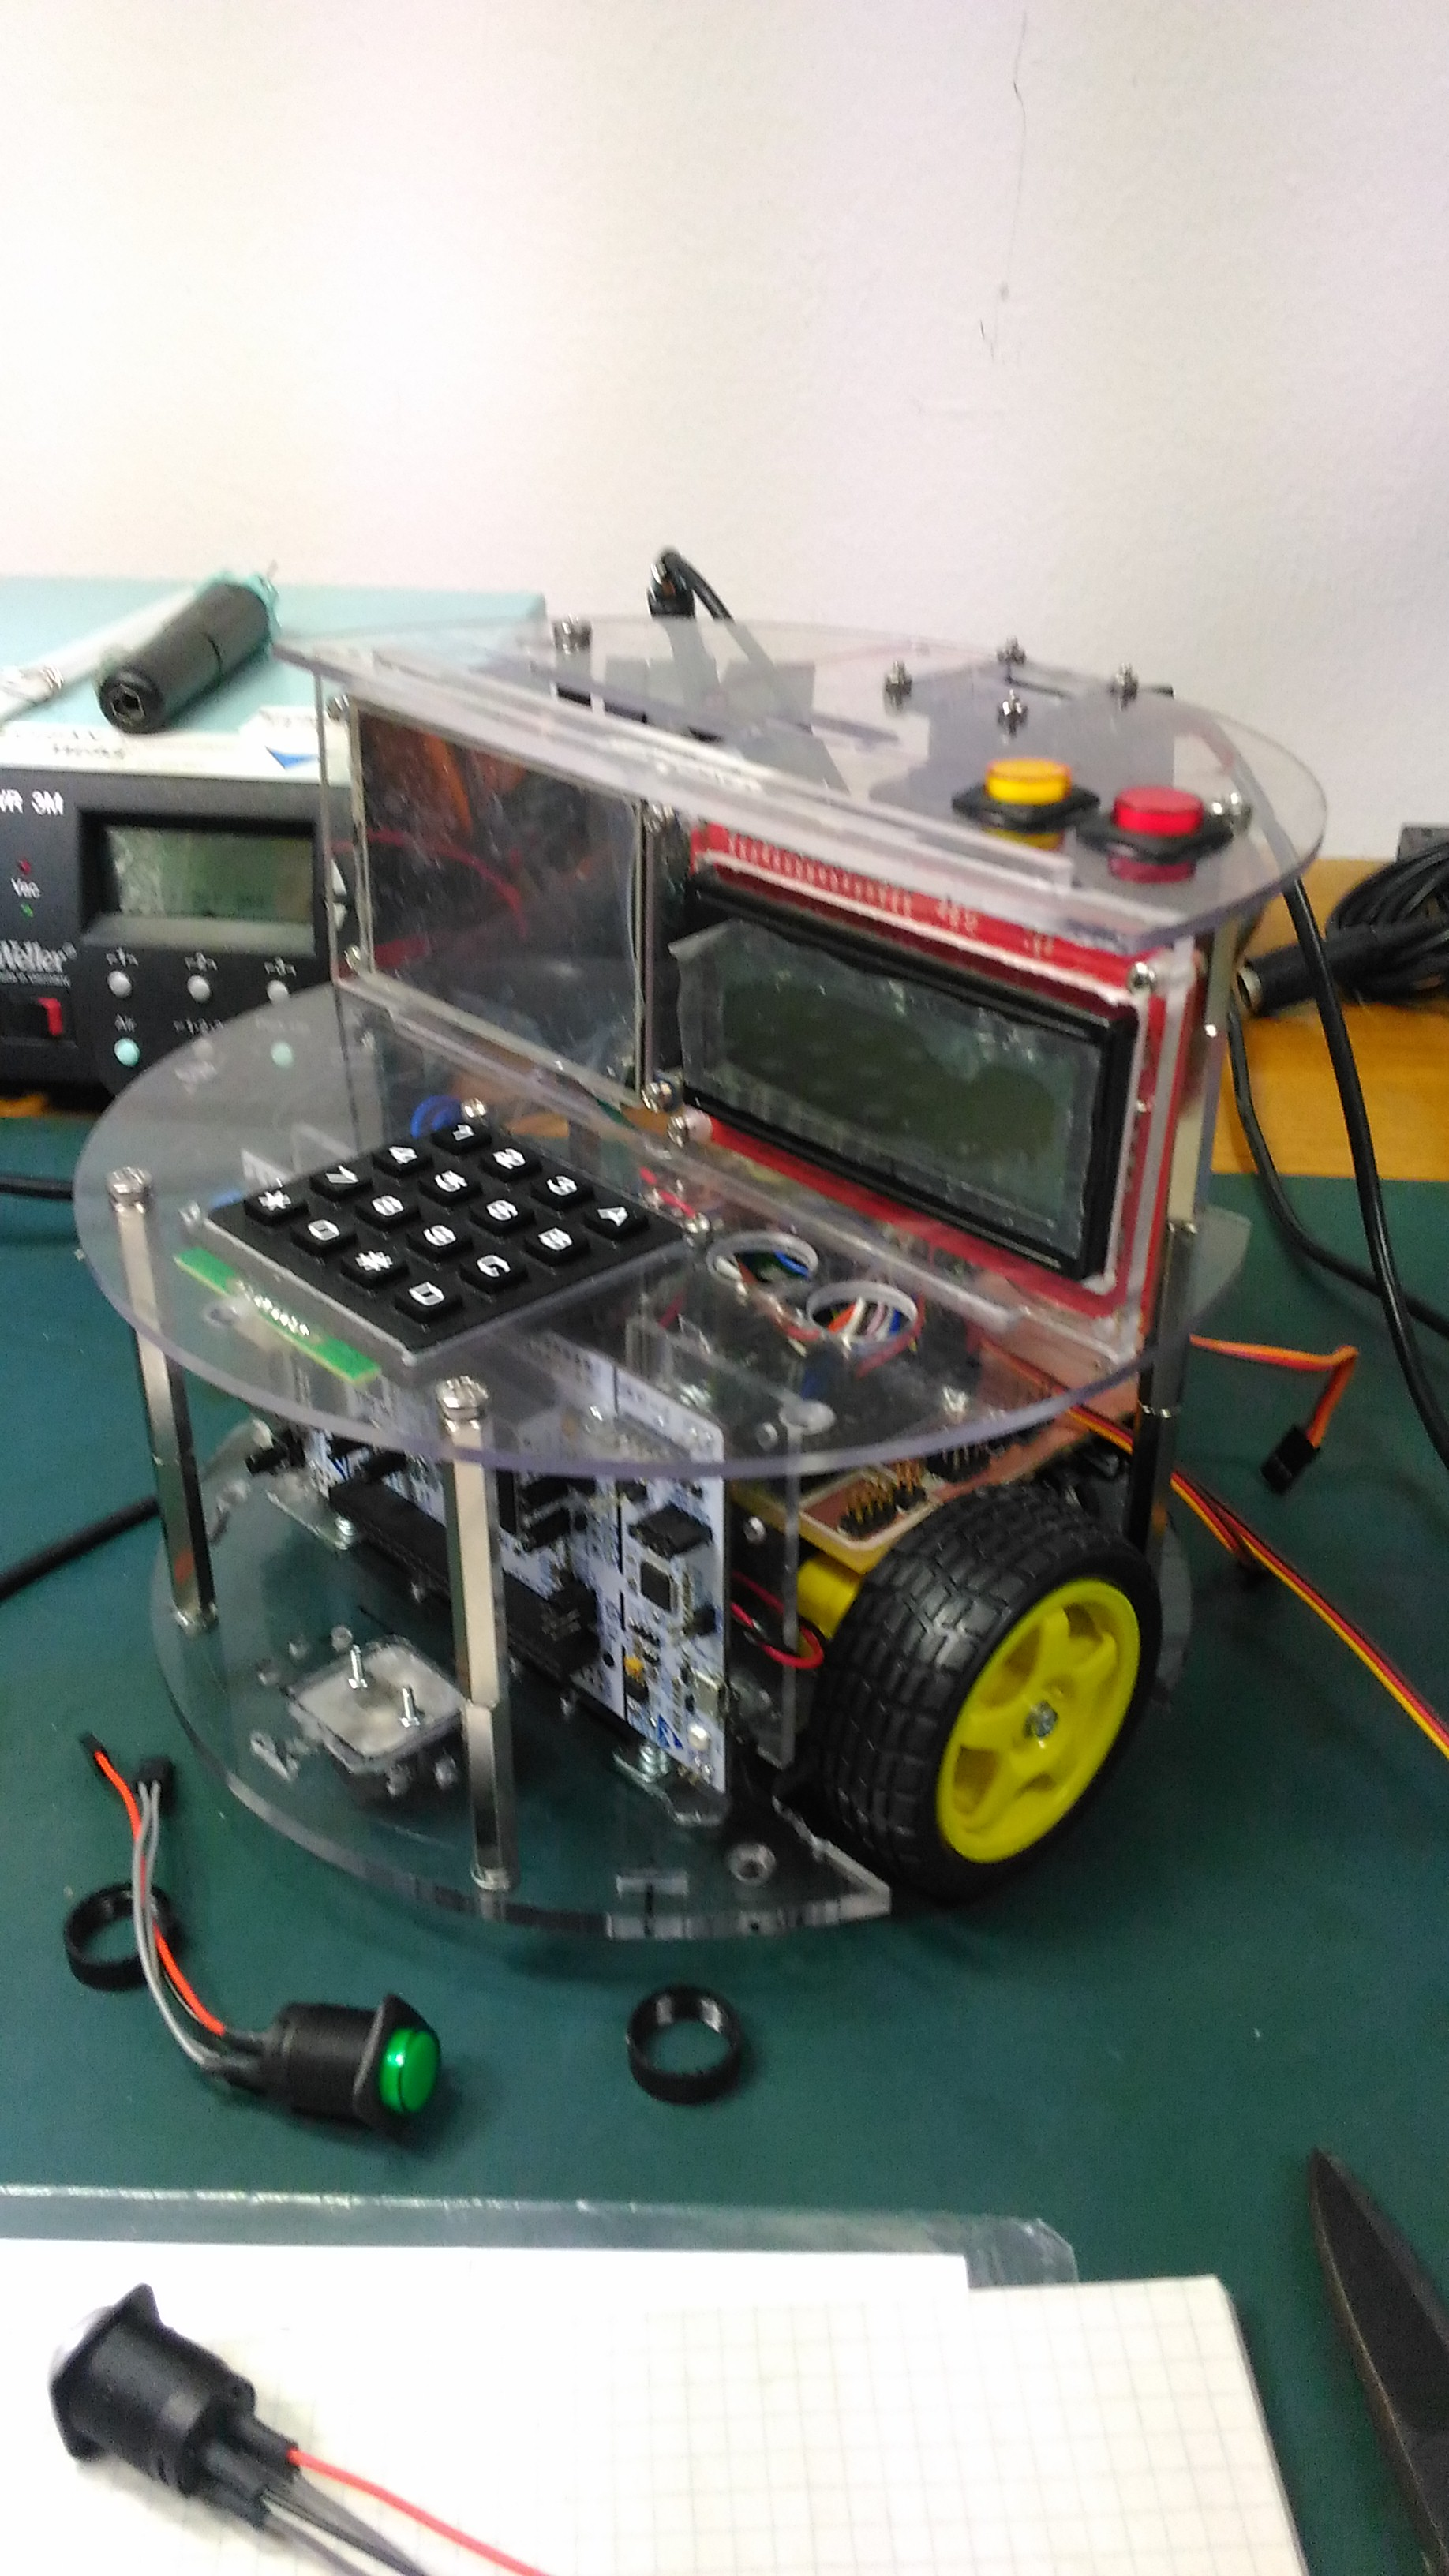
\includegraphics[width=0.3\textwidth,height=0.45\textwidth]{figures/turtlebot_1.jpg}
		\label{fig:tbot1}}
	\subfloat[The TurtleBot 2]
	{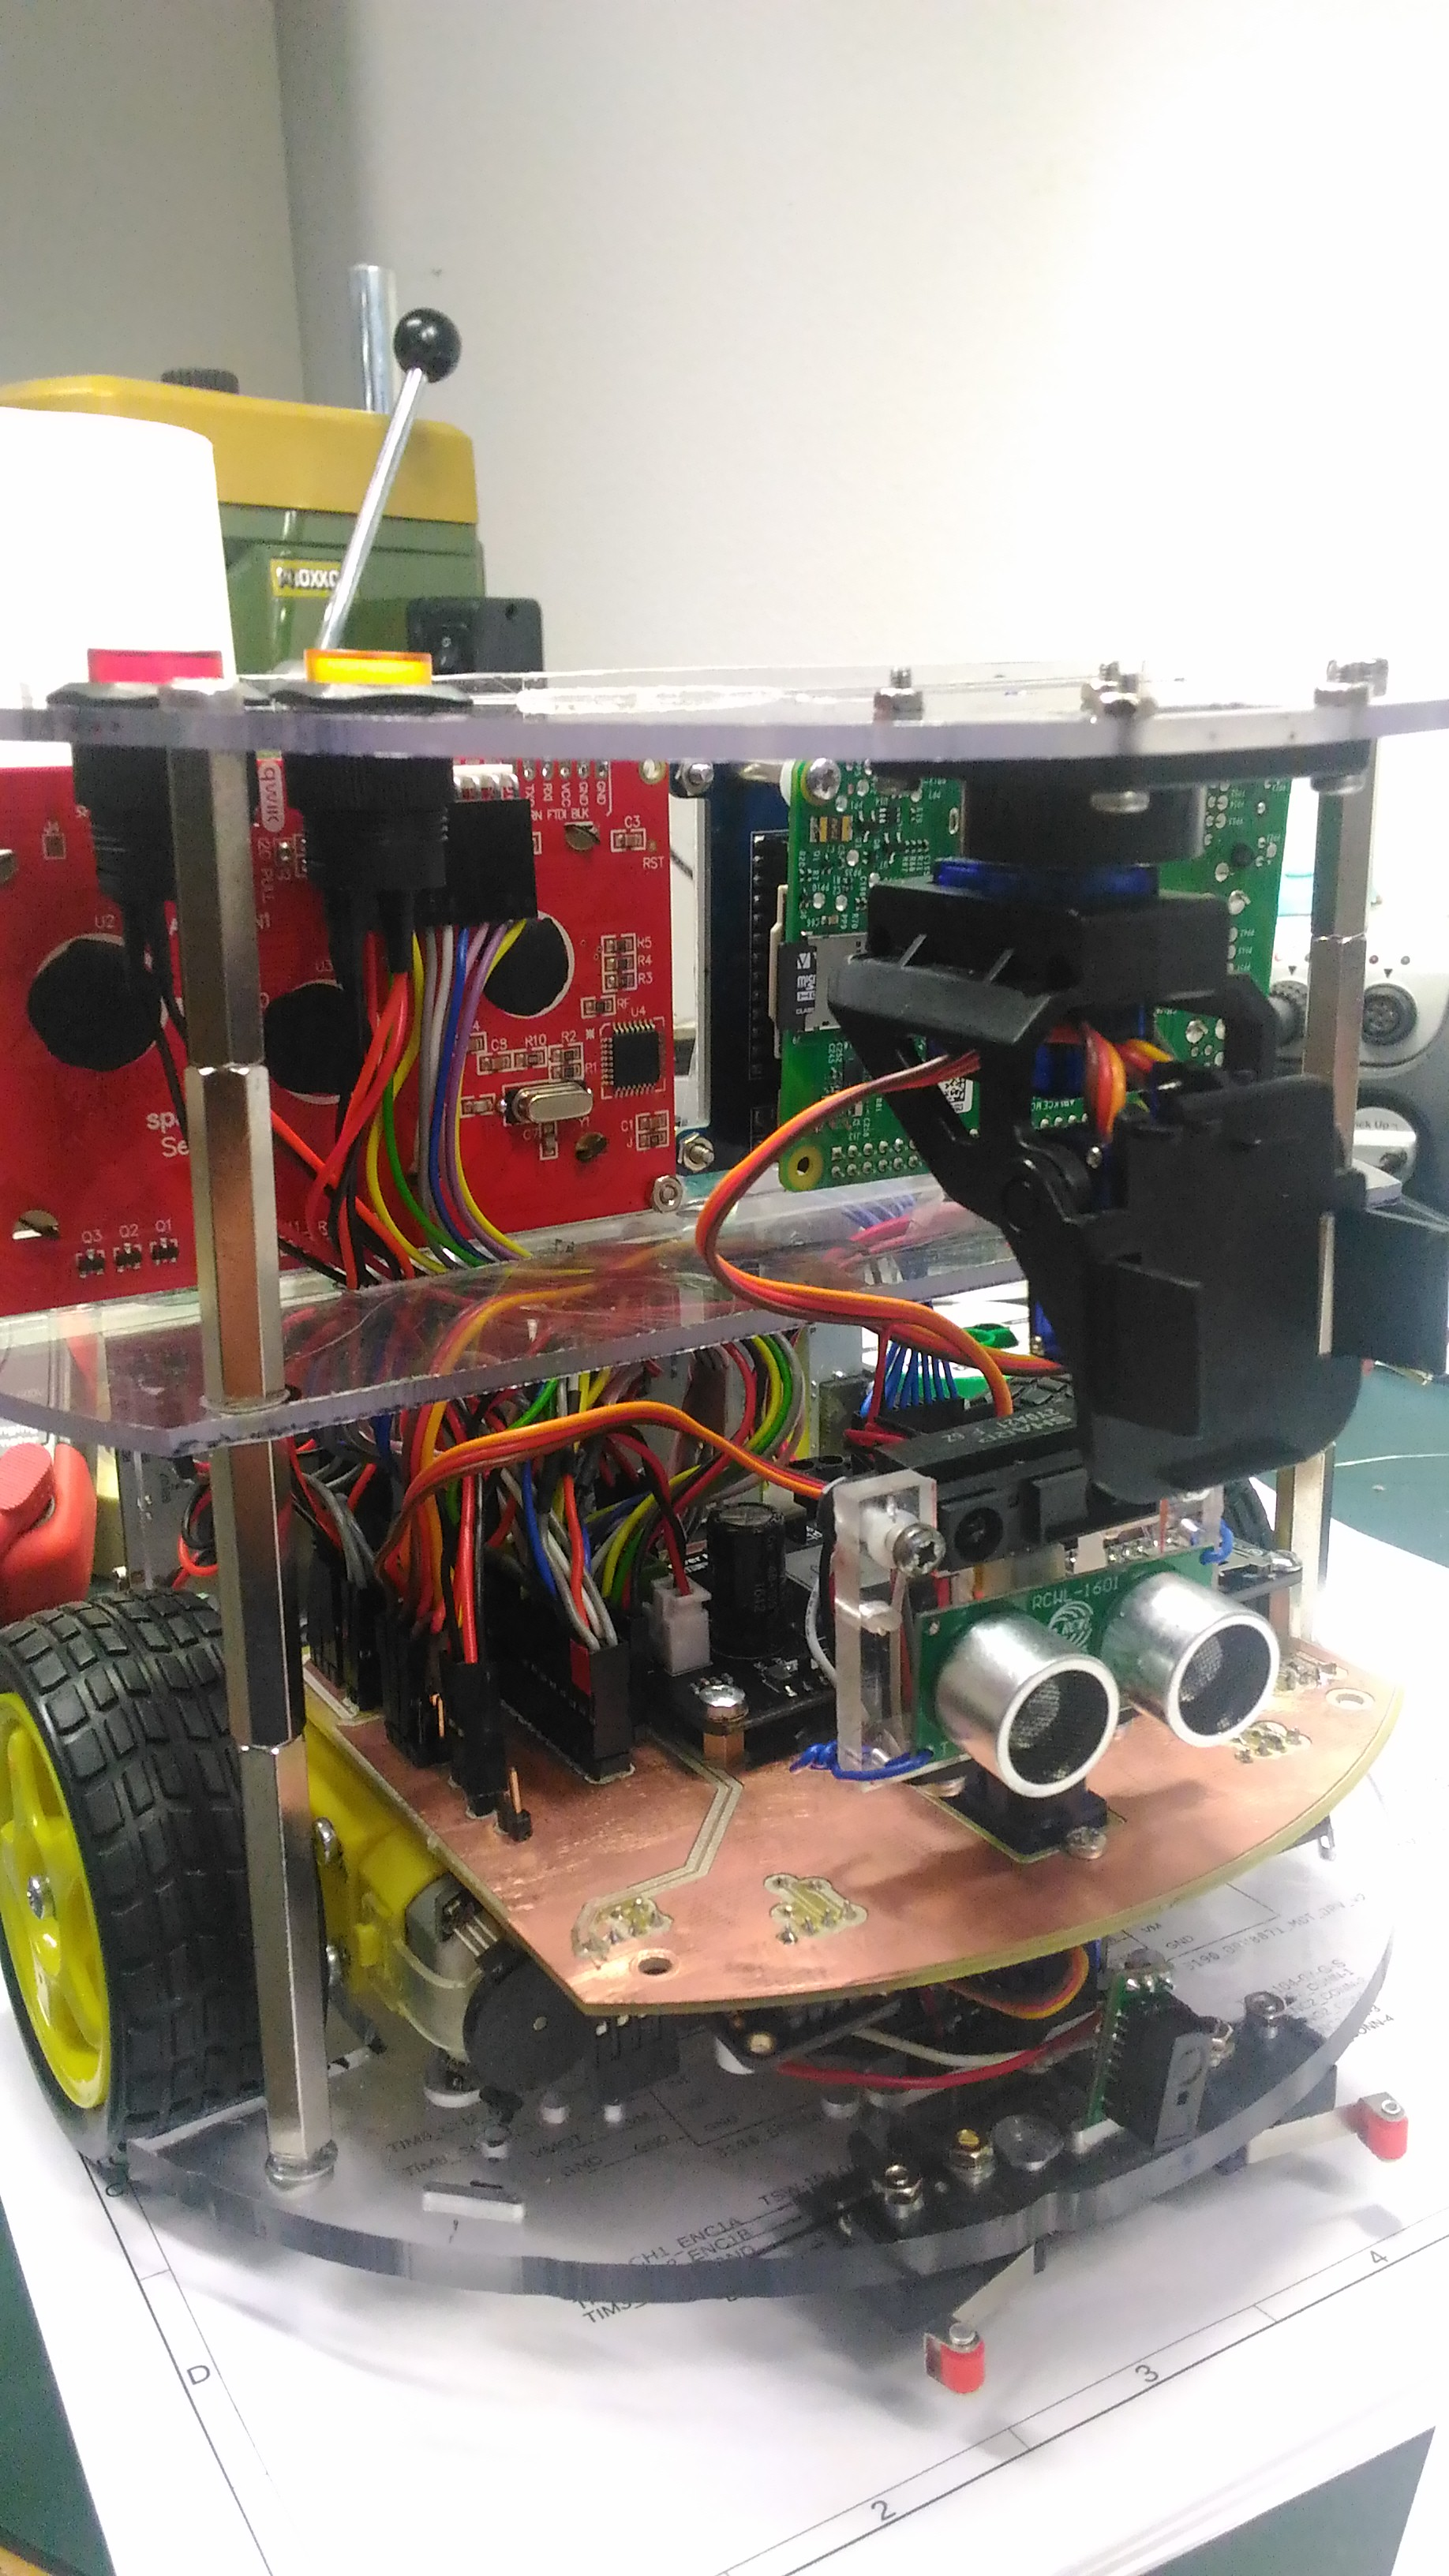
\includegraphics[width=0.3\textwidth,height=0.5\textwidth]{figures/turtlebot_2.jpg}
		\label{fig:tbot2}}
	\caption{The TurtleBot}
\end{figure}

\subsection{Another subsection}

Lorem ipsum dolor sit amet, consectetur adipisci elit, sed eiusmod tempor incidunt ut labore et dolore magna aliqua. Ut enim ad minim veniam, quis nostrum exercitationem ullam corporis suscipit laboriosam, nisi ut aliquid ex ea commodi consequatur.

\subsection{Another subsection}

\begin{lstlisting}[language=C, caption={C code using listings}, label={lst:label} ]
#include <stdio.h>
int main()
{
	// print hello to the console
	printf("Hello, world!");
	return 0;
}
\end{lstlisting}

See code~\ref{lst:label}.




\clearpage
\appendix

\section{Section in the Appendix}
\label{sec:app1}

\subsection{Subsection in the Appendix}
\label{subsec:app2}

Additional relevant information...

\end{document}